\documentclass[xcolor=dvipsnames]{beamer}
\useoutertheme{infolines}
\setbeamertemplate{navigation symbols}{}
\setbeamertemplate{items}[ball]
\usepackage{graphicx,multirow,color,xcolor,verbatim,float,comment,amsmath}
\setbeamertemplate{frametitle}[default][center]
\begin{document}
\title{Simultaneously Identifying Pathways via Multiple Value Genetic Algorithm}
\author{Bowen Deng}
\institute{Dept. of Prob. and Stat.}
\date{}
\begin{frame}
\maketitle
\end{frame}
\begin{frame}{Organization}
\tableofcontents
\end{frame}
\section{Literature Review}
\begin{frame}{Optimization Problem}
Objective:
\begin{displaymath}
\begin{split}
\max O(M_1,\cdots,M_t)&=\sum_{i=1,\cdots,t} W(M_i)\\
s.t. |M_i|&\in[k_{\min},k_{\max}]\\
M_i\cap M_j&=\emptyset
\end{split}
\end{displaymath}
\end{frame}
\begin{frame}{Binary Linear Programming}
\begin{displaymath}
\begin{split}
\max O(M_1,\cdots,M_t)=\sum_{\rho=1}^t\sum_{i=1}^m(2C_i(M_{\rho})&-\sum_{j=1}^nI_{M_{\rho}}(j)A_{ij})\\
s.t. \sum_{j=1}^nI_{M_{\rho}}(j)A_{ij}&\geqslant C_i(M_{\rho})\\
\sum_{\rho=1}^tI_{M_{\rho}}(j)&\leqslant 1\\
k_{\min}\leqslant \sum_{j=1}^nI_{M_{\rho}}(j)&\leqslant k_{\max}
\end{split}
\end{displaymath}
\end{frame}
\begin{frame}{MDendrix and IterDendrix}
To find $t$ pathways, one method is to solve the ILP directly. (MDendrix)\\
Another iterative approach is to solve the ILP with $t=1$, delete the identified genes, and run iteratively. (iterDendrix)\\
By theory, the time cost of MDendrix and iterDendrix is comparable with small $t$.\\
\begin{displaymath}
\begin{split}
TC(M)&\geqslant TC(\text{iter once})\\
&=\frac{\sum_{\rho=1}^tTC(\text{iter once})}{t}\\
&=\frac{TC(\text{iterDendrix})}{t}\\
&\geqslant \frac{TC(\text{mDendrix})}{t}
\end{split}
\end{displaymath}
\end{frame}
\begin{frame}
The authors used CPLEX v12.3 for implementation. We use lpSolve package in R. Set simulation data with $m=200$, $n=1000$, $I=10$, $t=3$. $k_{\min}=8$, $k_{\max}=12$.\\
MDendrix:\\
\begin{displaymath}
\begin{array}{ccc}
\text{Time Cost}&184.32&\\
\text{Result}&\text{Score}&\text{Score of Standard}\\
1\sim 10\,761\,774&30&32\\
11\sim 20\,752\,973&35&40\\
21\sim 30\,34\,109&32&36\\
\end{array}
\end{displaymath}
IterDendrix:\\
\begin{displaymath}
\begin{array}{ccc}
\text{Time Cost}&7.06&\\
\text{Result}&\text{Score}&\text{Score of Standard}\\
1\sim10\,214\,774&30&32\\
21\sim 30\,34\,109&32&36\\
11\sim 20\,652\,752&35&40
\end{array}
\end{displaymath}
\end{frame}
\section{Candidate Criteria}
\begin{frame}{Candidate Criteria}
For mutation matrix $A$, $p$ takes value in $m$ patients, and $g$ takes value in $n$ genes. $M$ is a set of genes.\\
We borrow the criteria from RME, an alternative approach for driver pathway identification.\\
Coverage Score:\\
\[C(M)=\frac{\#(\exists g\in M \text{ mutates in }p)}{m}\]
Exclusivity Score:\\
\[E(M)=\frac{\#(\text{exactly one } g\in M \text{ mutates in }p)}{\#(\exists g\in M \text{ mutates in }p)}\]
\end{frame}
\begin{frame}
Denote $I_M(p)$ the occurrence indicator of mutations of patient $p$ in $M$.\\
\begin{equation}
\begin{split}
S(M)&=C(M)+E(M)\\
&=\frac{\#\{I_M(p)>0\}}{m}+\frac{\#\{I_M(p)=1\}}{\#\{I_M(p)>0\}}\\
W(M)&=2\#\{I_M(p)>0\}-\sum_pI_M(p)\\
\end{split}
\end{equation}
The objective is to find $\hat{M}$ as the maximizer of $S(M)$. We could also restrict $|M|=k$.\\
\end{frame}
\begin{frame}{Simultaneous Detection with New Criteria}
We combine this new criteria with mDendrix to detect a mutually exclusive set of genes $M=\{M_1,\cdots,M_t\}$ which maximizes:
\[
S(M)=\sum_{\rho=1}^t S(M_{\rho})
\]
$k_{\min}\leqslant |M_{\rho}|\leqslant k_{\max}$.\\
\end{frame}
\section{Genetic Algorithm}
\begin{frame}{Computation}
The objective is to maximize $S(M)$. GA (Genetic Algorithm) is one of the top choices:\\
\begin{itemize}
\item The problem is no longer an BLP (Binary Linear Programming) task.\\
\item MCMC might trap in a local maxima.\\
\item The return value of GA is a set of solutions, suboptimal solutions are obtained as bonus.\\
\item GA's time cost is tractable.\\
\item GA is flexible for further integrated approach and variable scoring settings.\\
\end{itemize}
However, we should generalize the GA because it only works for binary case.\\
\end{frame}
\begin{frame}{Toy Example of GA}
We would like to maxmize $f(x)=e^{-x^2}, x\in[-5,5]$.\\
\begin{figure}
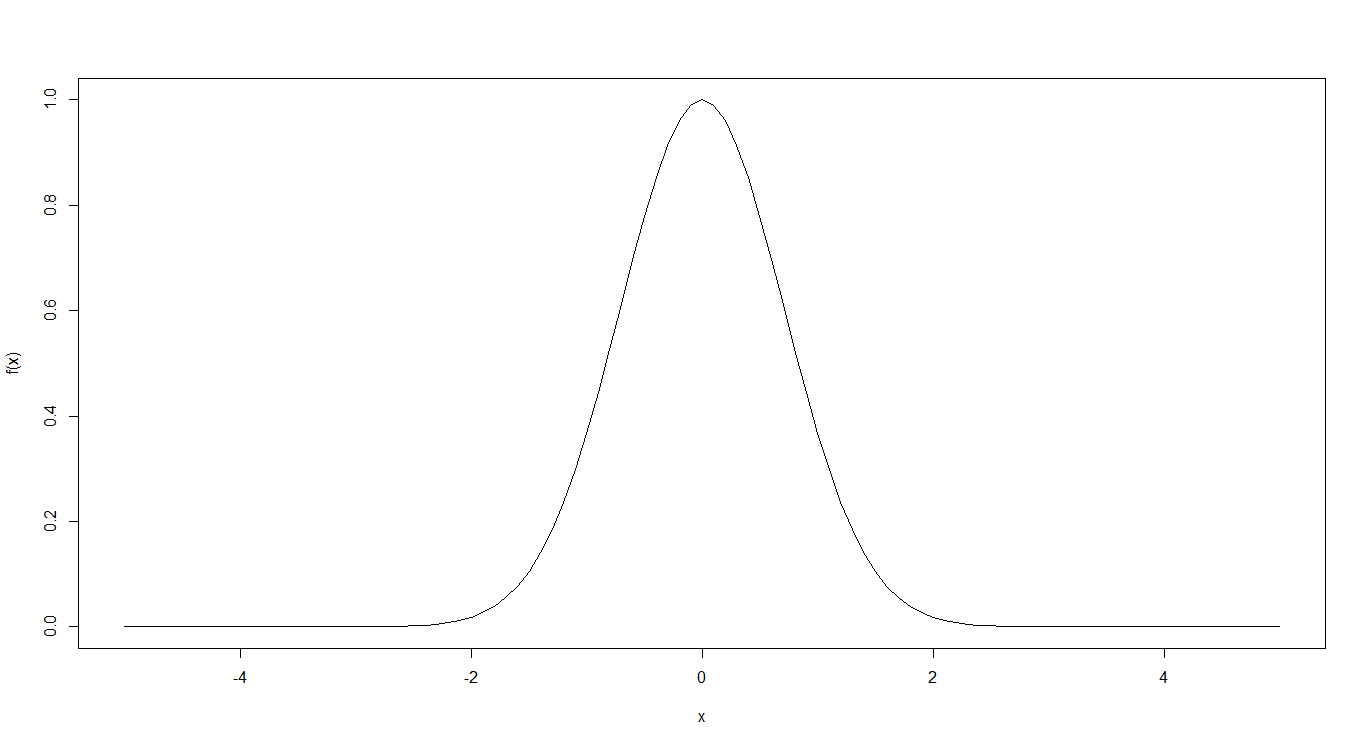
\includegraphics[width=0.9\linewidth]{toyfunction.png}
\caption{Objective Function}
\end{figure}
\end{frame}
\begin{frame}{Initialize a Population}
We first select a parent generation of size $P=10$ from $[-5,5]$.\\
2.42  2.33  2.04  2.00 -0.71  1.16 -1.16  1.75  3.66  4.20\\
\end{frame}
\begin{frame}{Crossproduct}
We select two of the parents to produce a child.\\
The probability of $x$ being selected is proportional to $f(x)$, therefore, an elite is more likely to be chosen than a normal person candidate.\\
The crossproduct is flexible with specific problems, here we could use $cp(x,y)=\frac{x+y}{2}$.\\
We generate $P=10$ children.\\
-0.938 -0.938  0.224 -0.938  0.224  0.811  0.224 -0.938 -0.938 -0.938
\end{frame}
\begin{frame}{Mutation}
With probability 0.1, a child will mutate if it increases its score.\\
\end{frame}
\begin{frame}{Iteration}
We pool the parents and the children and get 20 candidates.\\
We remain the 10 top scored ones.\\
0.224 -0.715  0.811 -0.938 -1.161  1.163  1.750  2.005  2.047  2.338 2.427  3.664  4.209\\
We use them to produce the next generation iteratively until convergence.\\
-7.24e-09  5.27e-09  2.85e-10 -9.82e-10 -5.02e-09 -3.48e-10 -7.14e-09  4.05e-09  2.78e-09 6.54e-09\\
\end{frame}
\begin{frame}{Analysis}
To improve the efficiency of Genetic Algorithm, i.e. the convergence rate, we should use large population size $P$, higher mutation rate (though a high mutation rate might increase the computation cost).\\
To avoid unnecessary computation, we set up a reasonable, rather than a perfect ending condition.\\
\end{frame}
\section{Multiple Value Genetic Algorithm}
\begin{frame}{MVGA}
We could generalize the GA algorithm to multiple value case.\\
Most steps are similar, but the crossproduction is much harder.\\
Let $k_{\min}=k_{\max}=2$,\\
Father:\\
11223300\\
Mother:\\
22331100\\
Their child should inherit two 1s, two 2s and two 3s. But the child should be as distinct from its parents as possible.\\
\end{frame}
\begin{frame}{Crossproduct}
Denote father: $F=(a_1,\cdots,a_n)$, mother: $M=(b_1,\cdots,b_n)$, $a_i,b_i\in\{0,1,\cdots,t\}$.\\
$a_i=\rho$ means i-th gene is in the $\rho$-th set, if $\rho=0$, i-th gene is not selected.\\
The motivation is to find a feasible solution corresponding to child $c_1,\cdots,c_n$ under constraint:\\
\[
\sum_{i=1}^n[(1-x_i)\mathrm{I}(a_i=\rho)+x_i\mathrm{I}(b_i=\rho)]\in[k_{\min},k_{\max}]
\]
where $x_i=0$ represents $c_i=a_i$, and $x_i=1$ represents $c_i=b_i$.\\
Moreover,\\
\[\sum_{a_i\text{ or }b_i>0}x_i\in[\frac{s-c}{2},\frac{s+c}{2}].\]
where $s=\#\{a_i\text{ or }b_i>0\}$.\\
We should minimize $c$ (ILP).\\
\end{frame}
\begin{frame}{Discussion}
At first glance, we plug an ILP inside of a genetic algorithm, the computation is expensive.\\
However, we only need to involve $|F\cup M|\leqslant 2tk_{\max}\ll n$ binary variables and one integer variable.\\
\end{frame}
\section{Parameter Selection}
\subsection{Selection of $t$}
\begin{frame}{Selection of $t$}
We set up a high score threshold $s_0$, a gene pathway $M$ is good if $S(M)>s_0$.\\
Release the constraint on the length of pathways found (although we set bounds wide enough for the sake of computation in real application), and we use MVGA to identify $t$ pathways $M_{\rho}^i$ which maximize $\sum_{\rho=1}^{t}S(M_{\rho})$ for $i=1,2,\cdots,\ell$.\\
We define RGP (rate of good pathway) as:
\[
\text{RGP}=\frac{\#\{W(M_{\rho}^i)>s_0\}}{\ell t}
\]
The RGP would decrease after the best $t$, and we could select the decreasing point as the estimation of $t$.\\
\end{frame}
\begin{frame}{Identifying the decreasing point of RGP}
\begin{figure}
\centering
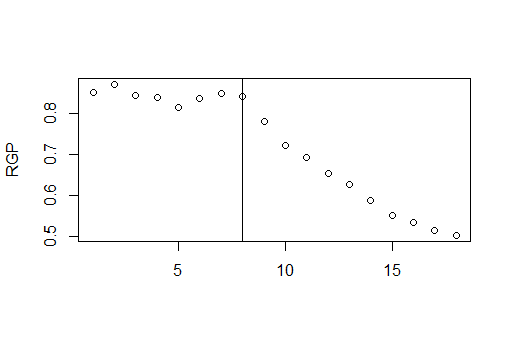
\includegraphics[width=0.9\linewidth]{RGP.png}
\caption{RGP in respect with t}
\end{figure}
\end{frame}
\begin{frame}
\begin{figure}
\centering
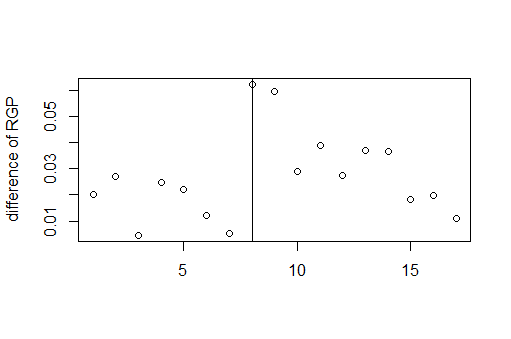
\includegraphics[width=0.9\linewidth]{diff.png}
\caption{difference of RGP in respect with t}
\end{figure}
\end{frame}
\begin{frame}
Based on these observations, we select the $t$ that maximizes $\frac{|x_{t+1}-x_t|}{|x_t-x_{t-1}|}$ as the final estimation.\\
\end{frame}
\subsection{Selection of range}
\begin{frame}{Selection of $k_{\min}$ and $k_{\max}$}
Once $t$ has been selected, we now need to estimate $k_{\min}$ and $k_{\max}$.\\
For the sake of computational cost, we constrain that $\ell(M_{\rho})\in[gk_{\min},gk_{\max}]$.\\
Assume
\begin{displaymath}
\Pr(\ell(M_{\rho})=x)=
\begin{cases}
\frac{q}{k_{\min}-gk_{\min}}&x\in[gk_{\min},k_{min})\\
\frac{1-2q}{k_{\max}-k_{\min}+1}&x\in[k_{\min},k_{\max}]\\
\frac{q}{gk_{\max}-k_{\max}}&x\in(k_{\max},gk_{\max}]
\end{cases}
\end{displaymath}
\end{frame}
\begin{frame}
where $gk_{\min}<k_{\min}\leqslant k_{\max}<gk_{\max}$.\\
We run $s$ results $x_{11},x_{12},\cdots,x_{st}$. Denote $l(x_{ij})=l_{ij}$.\\
The likelihood of $k_{\min}$ and $k_{\max}$ is
\[
L(k_{\min},k_{\max})=\prod_{1\leqslant i\leqslant s, 1\leqslant j\leqslant t}\Pr(\ell(M)=l_{ij})
\]
We use M.L.E. to estimate $\hat{k}_{\min}$ and $\hat{k}_{\max}$.
\[
(\hat{k}_{\min},\hat{k}_{\max})=\arg \max \ln L(k_{min},k_{\max})
\]
\end{frame}
\section{Further Work}
\begin{frame}{Further Study Directions}
\begin{itemize}
\item Find alternative crossproduct method for MVGA\\
\item Apply both simulation data and biological data to test the new method\\
\item Mathematically proof of the stability of parameter selection of $k_{\min}$ and $k_{\max}$\\
\end{itemize}
\end{frame}
\end{document}
